Randomness is extremely important in cryptography, and the same random values should never be used twice. It is hard to achieve, often we use pseudo-random number generators (PRNGs) to generate randomness. \\

\textbf{Example of Importance of Randomness:}
In a perfect secrecy scheme, the key is as long as the message. If the same key is reused even once, the messages can be decrypted. XORing their ciphertexts effectively removes the key, leaving a direct relationship between the two plaintexts. \\

For a message $m$ and key $k$, the ciphertext is $c = m \oplus k$, where $\oplus$ is the XOR-operation. For two messages encrypted with the same key:

\[c_1 = m_1 \oplus k\] 
\[c_2 = m_2 \oplus k\]

Now, if we XOR the ciphertexts:
\[c_1 \oplus c_2 = (m_1 \oplus k) \oplus (m_2 \oplus k)\]

Using the property of XOR that \(a \oplus a = 0\) and \(a \oplus b \oplus a = b\), we can deduce:

\[
c_1 \oplus c_2 = m_1 \oplus m_2 \oplus k \oplus k
\]

\[
c_1 \oplus c_2 = m_1 \oplus m_2
\]

Thus, the XOR of the two ciphertexts directly reveals the XOR of the two plaintexts. The ``distance" between two messages $m_1$ and $m_2$ represented by their XOR operation $m_1 \oplus m_2$, reveals the bitwise differences between them. This is often inpreted as the Hamming distance (the number of positions at which two strings of the same length differ) between the two messages. The XOR distance not only represents differences but can be exploited to reconstruct messages in insecure systems where the same key is reused (for instance, when the adversary knows one of the plaintexts already and can reconstruct the other).

\subsection{Stream Ciphers}

\begin{defn}
Stream ciphers are based on zeroes and ones. They encrypt bits (bit by bit) instead of blocks of plaintext. Due to bit operations, they are very fast. Easy to implement on hardware and software.
\end{defn}

Consider the following stream cipher:

\[ c = m \oplus F_k(0) \]

Where $F_k(0)$ is a function that generates a keystream based on the key $k$. The keystream is XORed with the plaintext to produce the ciphertext. The keystream is generated by a pseudo-random number generator (PRNG) that takes the key as input. \\

If the key was the same length of the message it would be perfect, but creating such a long key would be very inefficient (only done for government to government communication).
However, we can use a shorter key to mimic this behaviour. The short key is used to choose the output of a PRF (the key is the seed of the PRNG). It will mimic pseudo-randomness long enough (until it repeats itself). The cipher will be passive secure if the PRF is random enough.

\subsection{Linear Feedback Shift Registers (LFSRs)}
We can use LFSRs for generating a binary stream.

\begin{defn}
 A \textbf{Linear Feedback Shift Register} (LFSR) is a sequential shift register that generates a sequence of bits based on a linear feedback function. It consists of:
 \begin{itemize}
    \item A sequence of single-bit registers (0 or 1)
    \item Feedback function: a linear function (usually XOR) that determines how bits are fed back into the register.
    \item Tap positions in the register used in the feedback function.
 \end{itemize}
\end{defn}

\textbf{How it works:}
\begin{enumerate}
    \item Initialization: The register is initialized with a seed value (a non-zero starting state).
    \item Bit Shifting: The register shifts all bits to the right (or left), discarding the last bit.
    \item Feedback Calculation: A new bit is computed based on the XOR of the bits in the ``tapped'' positions.
    \item Repeat: The new bit is inserted into the first position of the register, and the process repeats to generate the next bit in the sequence.
\end{enumerate}

\begin{figure}[h!]
    \centering
    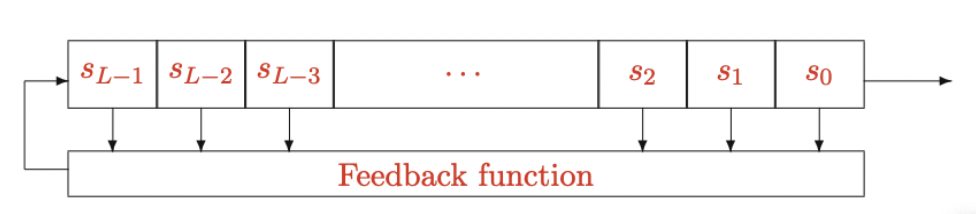
\includegraphics[width=0.5\textwidth]{img/LFSR.png}
    \caption{Feedback shift register}
\end{figure}

The initial state is very important, as it determines the entire sequence (whole sequence of zeroes always results in zeroes). The feedback function and length of the registers are also important.

\subsubsection{Properties of LFSRs}
\begin{itemize}
    \item Periodicity: LFSRs are periodic; they generate a sequence that eventually repeats. The maximum period is $2^n - 1$, where $n$ is the register size, achieved when the feedback taps correspond to a primitive polynomial.
    \item Deterministic: If the initial state (seed) and feedback function are known, the sequence is fully predictable.
    \item Efficiency: LFSRs are computationally efficient, using only shift and XOR operations.
\end{itemize}

\subsubsection{Feedback Functions}
Feedback functions in shift registers are used to compute the new bit that is fed back into the register. The key difference between linear and nonlinear feedback functions lies in how they combine the bits from the register.

\begin{table}[h!]
    \centering
    \renewcommand{\arraystretch}{1.2} % Adjust row spacing
    \begin{tabular}{|>{\raggedright\arraybackslash}m{4cm}|>{\raggedright\arraybackslash}m{5cm}|>{\raggedright\arraybackslash}m{5cm}|}
    \hline
    \textbf{Feature} & \textbf{Linear Feedback} & \textbf{Nonlinear Feedback} \\
    \hline
    \textbf{Operations} & XOR and other linear operations & Nonlinear operations (AND, OR, S-boxes, etc.) \\
    \hline
    \textbf{Predictability} & Easier to predict with known state & Harder to predict, more secure \\
    \hline
    \textbf{Efficiency} & Computationally efficient & More computationally intensive \\
    \hline
    \textbf{Periodicity} & Periodic, with a maximum of $2^n - 1$ & Can be non-periodic or have a very long period \\
    \hline
    \textbf{Applications} & Pseudo-random generators, CRC & Secure encryption, cryptographic systems \\
    \hline
    \end{tabular}
    \caption{Comparison of Linear and Nonlinear Feedback Functions}
    \label{tab:feedback_comparison}
\end{table}

We would like to have a non-linear feedback function, but these are difficult to design. Difficult to estimate whether it is a good non-linear function. When you hit 0 the whole value chain becomes 0, and the cycle is broken. \\

\subsubsection{Zero State in Feedback Functions:}
If an LFSR (or any shift register using feedback functions) reaches the value \textbf{zero}, the system will typically ``lock'' into this state and remain there indefinitely. This is because:

\begin{enumerate}
    \item Feedback Function Output: In a linear feedback system, the XOR of all zeros is zero, meaning that once all bits are zero, the feedback function will continue producing zeros.
    \item State Transition: The state of the LFSR will not change, and the register will stay stuck at zero, generating an output sequence that consists entirely of zeros.
\end{enumerate}

Implications:
\begin{itemize}
    \item \textbf{In LFSRs:}
    \begin{itemize}
        \item The sequence degenerates and loses all pseudo-randomness, becoming a constant stream of zeros.
        \item This reduces the period of the LFSR to just 1, which is undesirable, especially in cryptographic or pseudo-random number generation applications.
    \end{itemize}
    
    \item \textbf{In Cryptographic Systems:}
    \begin{itemize}
        \item If the feedback function hits zero during an encryption or random number generation process, it can render the output insecure.
        \item Attackers can easily exploit the fact that the system produces predictable, non-random output (all zeros).
    \end{itemize}
\end{itemize}

Avoiding the Zero State:
\begin{enumerate}
    \item Seed Initialization: The initial state (seed) of the register is carefully chosen to ensure it is non-zero.
    \item Primitive Polynomials: For LFSRs, the taps (feedback positions) are chosen based on primitive polynomials. This ensures the register cycles through all possible non-zero states ($2^n - 1$) before repeating.
    \item Nonlinear Feedback Functions: Nonlinear systems often include mechanisms to avoid degenerative states like zero, introducing additional complexity to prevent such behavior.
    \item External Checks: Some systems include checks to ensure that a zero state is never reached, restarting the LFSR with a valid non-zero state if necessary.
\end{enumerate}

\subsubsection{Mathematical Expression}
Cell is tapped or not (content of the cell contributes to the feedback function yes or no):
\[
[c_1, c_2, \dots, c_L]
\]

Initial state of the registers:
\[
[s_{L-1}, \dots, s_1, s_0]
\]

Output:
\[
[s_0, s_1, s_2, s_3, \dots, s_{L-1}, s_L, s_{L+1}, \dots]
\]

Then, for \(j \geq L\):
\[
s_j = c_1 \cdot s_{j-1} \oplus c_2 \cdot s_{j-2} \oplus \cdots \oplus c_L \cdot s_{j-L}.
\]

However, we need to see a repetition after a certain period, \(N\), such that:
\[
s_{N+i} = s_i.
\]

\(N\) can be maximum \(2^L - 1\). \\

The \textbf{connection polynomial} $C(X)$ describes how the bits stored in the LFSR are combined to produce the feedback bit, which determines the next state of the LFSR. It is defined as:

\[ C(X) = 1 + c_1 \cdot X + c_2 \cdot X^2 + \dots + c_L \cdot X^L \in \mathbb{F}_2\left[X \right] \]

where $\mathbb{F}_2\left[X \right]$ is the set of polynomials over the binary field (coefficients are either 0 or 1). Proper choice of $C(X)$ can result in a maximal period of $2^L - 1$.\\

The \textbf{characteristic polynomial} $G(X)$ describes the LFSR's output sequence and the polynomial that can be used to generate the entire sequence of output bits. It is a function of the feedback logic defined by the connection polynomial.

\[ G(X) = X^L \cdot C(1/X) \]

\textbf{Example:}

\begin{figure}[h]
    \centering
    \begin{subfigure}{0.45\textwidth}
        \centering
        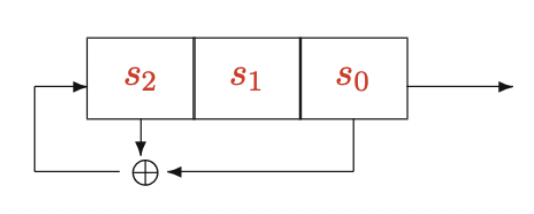
\includegraphics[width=\textwidth]{img/lfsr1.png}
        \caption{$X^3 + X + 1$}
    \end{subfigure}
    \hfill
    \begin{subfigure}{0.45\textwidth}
        \centering
        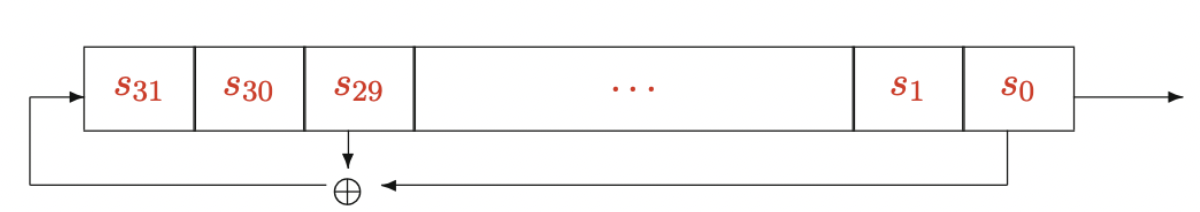
\includegraphics[width=\textwidth]{img/lfsr2.png}
        \caption{$X^{32} + X^3 + X + 1$}
    \end{subfigure}
    \caption{Linear Feedback Shift Register Examples}
    \label{fig:lfsr-examples}
\end{figure}

\begin{itemize}
    \item[a)] This is a small LFSR with length $L=3$, described by the connection polynomial $C(X) = X^3 + X + 1$. There are 3 registers: $s_0, s_1, s_2$. The feedback function involves: $X^3$ (feedback from the last register), $X$ (feedback from the first register), and a constant 1. At each step, the contents of the tapped cells ($s_2, s_0$) are XOR-ed to produce a new bit.
    \item[b)] This is a much larger LFSR with length $L=32$, described by the connection polynomial $C(X) = X^{32} + X^3 + X + 1$. There are 32 registers. The feedback function involves the 32nd (last) register, the 3rd register, the 1st register, and a constant 1. The characteristic polynomial $G(X)$ is used to generate the entire output sequence. \Comment{I dont get the exp values for this one??}
\end{itemize}

Note: The connection polynomial determines which registers contribute to the feedback. But is not a direct description of the output stream itself. Instead, it describes the feedback mechanism of the LFSR. \\

How do we know that the feedback function is a good one, such that we achieve the maximum length before the stream cipher repeats itself?

\subsubsection{Primitive Polynomial}
\begin{defn}
A \emph{primitive polynomial} is a polynomial that generates a maximal-length sequence in a finite field, particularly in the context of binary fields $\mathbb{F}_2$ (i.e., polynomials whose coefficients are either 0 or 1). Specifically, for a polynomial to be \textit{primitive}, it must satisfy the following conditions:

\begin{itemize}
    \item The polynomial must be \textbf{irreducible} over $\mathbb{F}_2$ (i.e., it cannot be factored into the product of lower-degree polynomials with coefficients in $\mathbb{F}_2$).
    \item The polynomial must generate a sequence that cycles through all the nonzero elements of the finite field $\mathbb{F}_{2^L}$, where $L$ is the degree of the polynomial.
\end{itemize}
    
In simpler terms, a primitive polynomial produces a sequence of numbers that goes through all possible states except the zero state (when viewed as an LFSR) before repeating.
\end{defn}

When used in LFSRs, primitive polynomials ensure that the generated sequence has a \emph{maximum length} before it repeats. The length of the sequence is $2^L -1$, where $L$ is the degree of the polynomial.

\begin{thm}
    If N is the period, then the characteristic polynomial $f(x)$ is a factor of $1-X^N$. 
\end{thm}


\[ C(X) = 1 + c_1 \cdot X + c_2 \cdot X^2 + \dots + c_L \cdot X^L \in \mathbb{F}_2\left[X \right] \]

Conditions for $C(X)$:
\begin{itemize}
    \item The highest coefficient $c_L$ = 0: the polynomial is singular. This means that $C(X)$ is not a full degree of $L$ and cannot properly generate sequences of maximal length in an LFSR.
    \item The highest coefficient $c_L$ = 1: the polynomial is non-singular. $C(X)$ is a full degree of $L$ and there is a periodicity in the sequences generated by the polynomial. The behaviour of the sequence depends on whether $C(X)$ is irreducible or not.
\end{itemize}

$C(X)$ is irreducible if it cannot be factored into smaller polynomials over $\mathbb{F}_2\left[X \right]$ (other than itself and 1).
Then, the period of the sequence generated by the LFSR is the \emph{smallest} N such that $C(X)$ divides $1 + X^N$.
$N$ will satisfy $N | (2^L-1)$. \\

\textbf{Example:}
3 registers, maximum length is 7:
\[m = 3, p = 2^3 -1 = 7\] 
So we need to find the factors of:
\[1 - x^y = (1-x)(1 + x + x^3)(1 + x^2 + x^3)\]

The divisors of this polynomial (irreducible polynomials) will have a period of 7.

\subsection{Period}

The presence of disjoint cycles in an LFSR, such as in figure \ref{fig:lfsr-period}, has implications for randomness:

\begin{figure}[h]
    \centering
    \begin{subfigure}{0.45\textwidth}
        \centering
        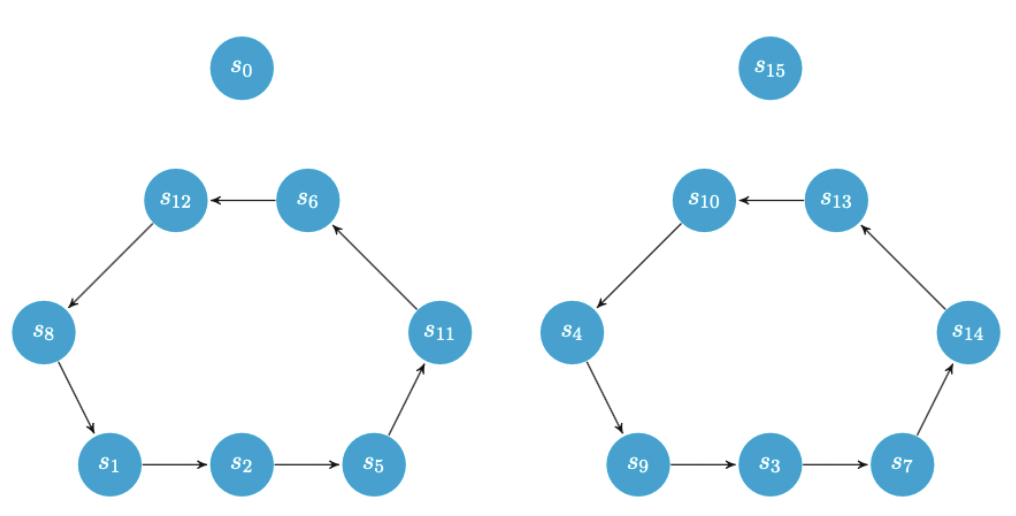
\includegraphics[width=\textwidth]{img/lfsrperiod1.png}
        \caption{$X^4+X^3 + X^2 + 1$}
    \end{subfigure}
    \hfill
    \begin{subfigure}{0.45\textwidth}
        \centering
        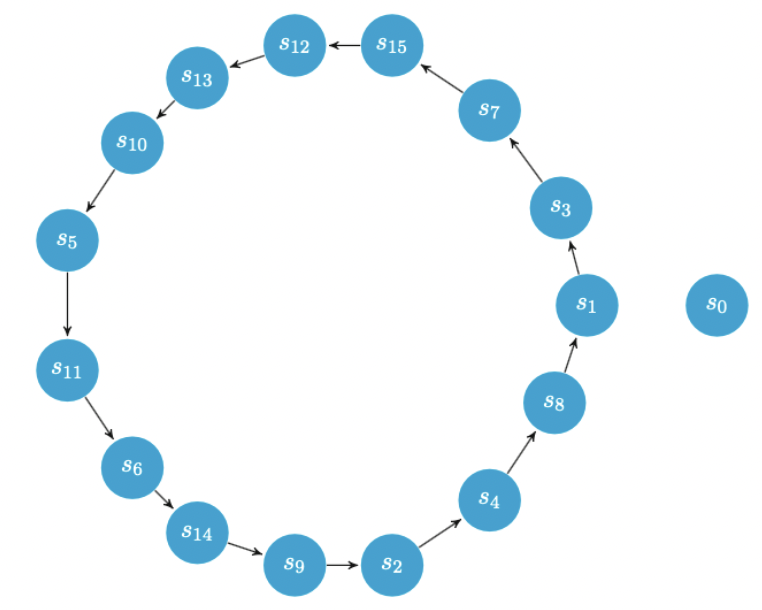
\includegraphics[width=\textwidth]{img/lfsrperiod2.png}
        \caption{$X^4 + X + 1$}
    \end{subfigure}
    \caption{State transitions of 4-bit LFSRs with connection polynomials}
    \label{fig:lfsr-period}
\end{figure}

\begin{itemize}
    \item The output sequence splits into two disjoint cycles of length 7 instead of a single cycle of length \( 2^L - 1 \) (15 for \( L = 4 \)).
    \item Reduced Period: The sequence repeats earlier, reducing the overall period and uniformity.
    \item Loss of Randomness: Missing states lead to gaps, making the sequence predictable and non-random.
    \item Cause: The connection polynomial is \textit{not primitive}, preventing the LFSR from achieving a maximum-length sequence.
\end{itemize}

The right polynomial results in a big cycle with all states included, except for the zero state, as expected.

\subsection{Security of LFSRs}
With $L$ registers and $2L$ known output bits, the connection polynomial can be revealed. It is a linear system. If you have sufficient equations, you can solve the linear system.
\begin{itemize}
    \item First $L$ bits reveal the $s$ values
    \item We need to learn $L$ unknowns: $c$ values
\end{itemize}

\[ s_j = \sum^L_{i=1} c_i \cdot s_{j-i} \pmod{2} \]

Therefore, LFSRs are not secure!

\Comment{Linear complexity notes here}

\subsection{Combining LFSRs}
LFSR-based stream ciphers are very fast ciphers, suitable for implementation in hardware, to encrypt real-time data such as voice or video. But they need to be augmented with a method to produce a form of non-linear output.

Create fast and secure non-linear behaviour by combining multiple LFSRs into a non-linear combination function: 

\begin{figure}[h!]
    \centering
    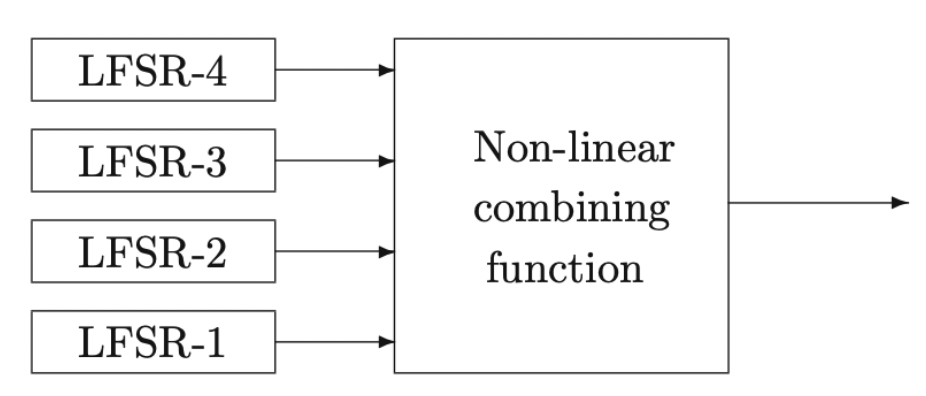
\includegraphics[width=0.5\textwidth]{img/combinelfsr.png}
    \caption{Combining LFSRs}
\end{figure}

\subsubsection{Non-linear Combiners}
Examples covered in lecture are:
\begin{itemize}
    \item Alternating-step generator
    \item Shrinking generator
    \item A5/1
    \item Trivium
    \item RC4
\end{itemize}
\Comment{How much do we need to know about these?}